\chapter{Sharding: Scaling Storage, Computation and Communication}

\section{Introduction}
Let's say two things:
\textbf{Bitcoin uses full replication:} In traditional blockchains like Bitcoin, the number of participants does not affect the load per node significantly because everyone stores, validates, and communicates every block. This leads to linear growth in the total load of the network as the number of participants increases, which can be resource-intensive and costly.\\
However, in distributed systems, achieving horizontal scaling is desirable. Horizontal scaling means that the performance of the system, such as the number of transactions processed or files distributed, scales linearly with the number of participating nodes. An example of horizontal scaling is the BitTorrent protocol for file-sharing, whereas more nodes join the network, the number of nodes storing a particular file increases, reducing the load per file request.\\
To achieve horizontal scaling in blockchains while maintaining consensus on the ledger order, the concept of sharding is used. Sharding involves splitting the database (ledger) into subsets, with each subset stored and managed by a different subset of nodes. This approach allows for full horizontal scaling, as not all nodes need to see and process all transactions. Instead, each node is responsible for a specific subset of transactions, allowing for better resource utilization and scalability.\\
The lecture focuses on the principled approach to sharding in blockchains, aiming to achieve full horizontal scaling without compromising on consensus and security. Sharding is a promising solution to address the resource burden and scalability challenges faced by traditional blockchain systems.\\
\textbf{First order approach to Sharding} In this first-order approach to sharding, the ledger is divided into K exclusive and non-intersecting subsets, each representing an independent application with its own transactions. These subsets are called shards, and the idea is to manage each shard as an independent blockchain. Each shard operates with its own consensus protocol, such as the longest chain protocol, and is maintained by N/K nodes out of the total N participating nodes in the network.\\
This approach achieves a form of horizontal scaling because each node is responsible for maintaining only one shard, which is a fraction 1/K of the entire ledger. Consequently, the maintenance costs, including storage, computation, validation, and communication, are reduced to 1/K of the overall ledger. As a result, the system can scale efficiently, and K can increase linearly with the number of participating nodes N, achieving optimal horizontal scaling.\\
However, this increase in efficiency and horizontal scaling comes at the cost of reduced security. The overall security of the system is limited by the security of any single shard, as an adversary can target and tamper with the state of the blockchain by attacking just one shard. Since each shard is maintained by a smaller subset of nodes (N/K nodes), attacking a single shard is easier for the adversary compared to attacking a single blockchain maintained by all N nodes.\\
In summary, the first-order approach to sharding provides K-fold horizontal scaling, but it decreases security by a factor of K. The challenge is to design a sharding mechanism that achieves horizontal scaling without compromising on security, which is the focus of the lecture. The lecture explores ways to provision horizontal scaling in blockchains while ensuring robust security for the entire system, even in the presence of adversarial attacks.
\section{Multiconsensus architecture} 
In this extended approach to sharding, the allocation of nodes to shards is done uniformly at random. An important aspect is that adversaries are no longer able to concentrate on a single shard to attack it. This is achieved through a cryptographically secure oracle that assigns nodes to shards randomly and fairly, and all participants can verify the correct allocation. This prevents adversarial collusion and maintains security even if a majority of honest nodes exist globally.\\
To enable random reallocation, a node-to-shard allocation engine (N2S) is introduced. The N2S is responsible for generating cryptographically secure random allocations of nodes to shards. This allocation can be managed by a separate service or as part of the blockchain itself. One approach is to use a distributed randomness generator like RandHound to create the randomness required for the allocation. Another method is to use a "beacon" consensus engine shared across all shards, which generates a shared distributed randomness. The beacon only contains state commitments and N2S allocation metadata, making it lightweight and easy for all nodes to maintain.\\
While this solution achieves horizontal scaling, it comes with some limitations:
\begin{enumerate}
    \item The N2S allocation requires each node to have an identity, making this sharding procedure not permissionless, which is different from Bitcoin's design.
    \item To maintain the fraction of honest hashing power in each shard and ensure the global majority of honest hash power translates to the majority honest hash power in each shard, the number of nodes per shard needs to be substantial, limiting the number of shards ($K$) as a function of the number of nodes ($N$), see Figure \ref{fig:f1}.
    \item The architecture is not secure against an adaptive adversary, as the adversary can corrupt miners after they have been allocated to a shard, leading to collusion within a shard. To address this, regular reallocations of N2S allocations can be conducted to prevent coordination and collusion by the adversary. However, faster rotations of allocations may introduce more overhead in the N2S procedure, which diminishes the horizontal scaling effect.
\end{enumerate}
These limitations are addressed in a full sharding solution, which is described next.
\begin{center}
    \begin{figure}
        \centering
        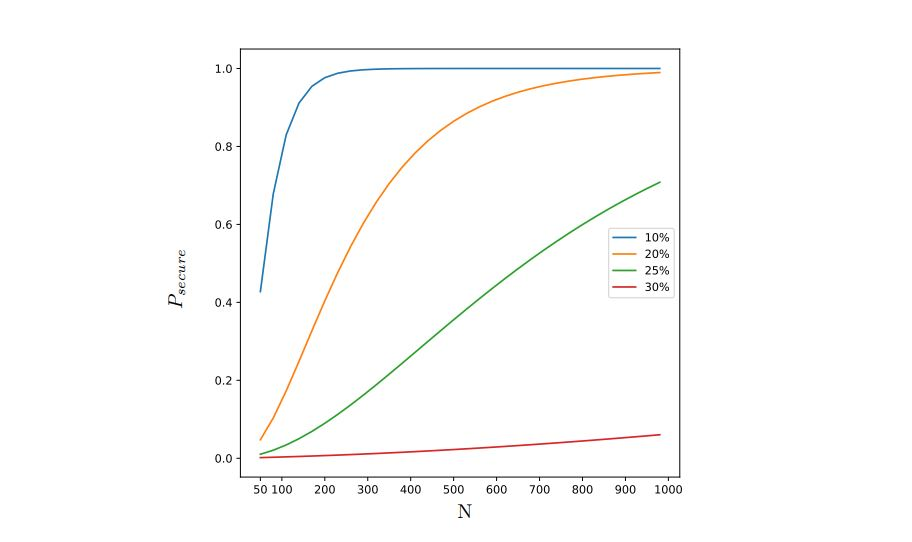
\includegraphics[width=0.8\linewidth]{Fig/10/F1}
        \caption{Probability that every shard is secure (i.e., an honest supermajority in each of the $K = 10$ shards) as a function of the number of users N under different adversarial models ($10\%$, $20\%$, $25\%$ and $30\%$ net adversarial fraction)}
        \label{fig:f1}
    \end{figure}
\end{center}
\section{Uniconsensus architecture}
In the uniconsensus architecture, the security properties of the multiconsensus approach are significantly improved by having every node participate in a single main consensus engine. This means that all nodes work together in the main consensus to maintain each shard, unlike the previous approach where only a small subset of nodes maintained a shard.\\
In this architecture, each node participates in a single main consensus engine, while also choosing a shard of its choice to mine shard blocks. This self-allocation of shards allows for better scalability and efficiency. The main consensus engine only maintains a log of the hash of shard blocks, which keeps it lightweight and easy for every node to maintain.\\
The coupling of shard blocks with the main consensus engine and ensuring adversary resistance is achieved through the same scaling principles we have seen in previous lectures. Specifically, the concept of "many-for-one mining" of a superblock and cryptographic sortition into constituent sub-blocks is utilized.\\
In other words, nodes work together to mine a superblock, which contains multiple shard blocks. This superblock is then cryptographically sorted into its constituent sub-blocks, each corresponding to a specific shard. This process ensures that shard blocks are securely integrated into the main consensus engine, and the cryptographic sortition adds a layer of protection against adversaries.
In the uni-consensus architecture, the data structure consists of two main types of block structures: a proposer block tree and $K$ shard ledgers.\\
\begin{itemize}
    \item \textbf{Proposer Blocktree:} The proposer blocktree is responsible for the single main consensus engine in the uniconsensus architecture. It is organized using a Proof-of-Work (PoW) based Nakamoto longest chain consensus protocol. Proposer blocks are the building blocks of this tree and contain the necessary information for the main consensus. Each proposer block also includes hash-pointers to shard blocks.
    \item \textbf{Shard Ledgers:} There are K shard ledgers, where K represents the number of shards. Each shard ledger consists of shard blocks. Shard blocks are specific to individual shards and are identified by their ShardID. These shard blocks contain shard transactions, similar to transaction blocks in the Prism protocol (as discussed in Lectures 8 and 9). Unlike the proposer blocktree, shard blocks do not contain any blocktree pointers, see Figure \ref{fig:f2}.
\end{itemize}
The absence of blocktree pointers in shard blocks is deliberate and serves a specific purpose. The ordering of shard blocks is solely inferred from their order in the main consensus engine, which is the longest chain of the proposer block tree. This is similar to the way the Prism protocol determines the ordering of transaction blocks without relying on blocktree pointers. In the uni-consensus architecture, the main consensus engine's longest chain of proposer blocks is used to order shard blocks within each shard.\\
The primary responsibility of shard block mining in this architecture is to ensure adversary resistance, ensuring that the blocks remain secure against attacks. However, shard block mining does not play a role in determining the ordering of shard blocks. Instead, their ordering is entirely derived from their corresponding hash pointers in the proposer chain.
\begin{center}
    \begin{figure}
        \centering
        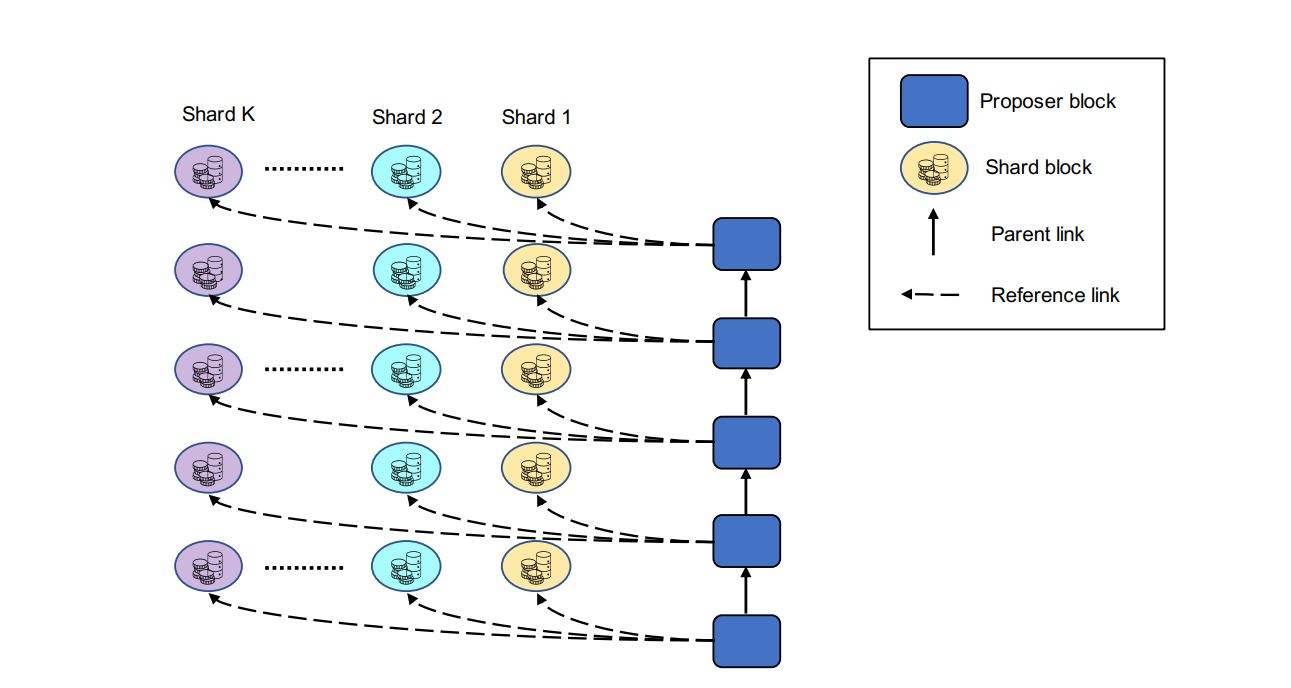
\includegraphics[width=0.8\linewidth]{Fig/10/F2}
        \caption{Data structures in the Uniconsensus architecture.}
        \label{fig:f2}
    \end{figure}
\end{center}
In this architecture, security is ensured by requiring every miner to mine both proposer blocks and shard blocks simultaneously. This is achieved through a process called "many-for-one mining" and cryptographic sortition.
\textbf{Many-for-One Mining: }Each mining node creates a superblock that contains a potential shard block for a specific shard of the node's choice, along with a potential proposer block. The miner then mines a nonce on the header of this superblock, which includes hash commitments of both the potential shard block and the potential proposer block. The miner's goal is to find a nonce such that the resulting hash of the superblock falls within certain predefined ranges.\\
\textbf{Cryptographic Sortition: }The cryptographic sortition algorithm ensures that the hash of the superblock falls within specific ranges, allowing it to be classified as either a proposer block or a shard block. Specifically, if the hash of the superblock falls between 0 and $\tau_{1}$ ($\tau_{1}$ represents the proposer block mining difficulty), then the superblock is treated as a proposer block. On the other hand, if the hash falls between $\tau_{1}$ and $\tau_{2}$ (where $\tau_2$ is a shard-specific variable), the superblock is treated as a shard block for the identified shard.\\
The combination of many-for-one mining and cryptographic sortition prevents adversaries from selectively focusing their mining resources solely on mining either proposer blocks or shard blocks. This ensures a fair distribution of mining efforts and contributes to the security of the system.\\
Moreover, during the mining process, the shard ID of the potential shard block is fixed, which means that a single mining attempt can only create a shard block for one specific shard (chosen by the miner). This helps maintain the integrity and separation of different shards in the system, This 2-for-one PoW sortition
is shown in Figure \ref{fig:f3}.\\
To maintain a consistent shard block generation rate for each shard, the shard block mining difficulty is periodically adjusted for each shard. This adjustment ensures that each shard generates blocks at a constant and controlled rate.
\begin{center}
    \begin{figure}
        \centering
        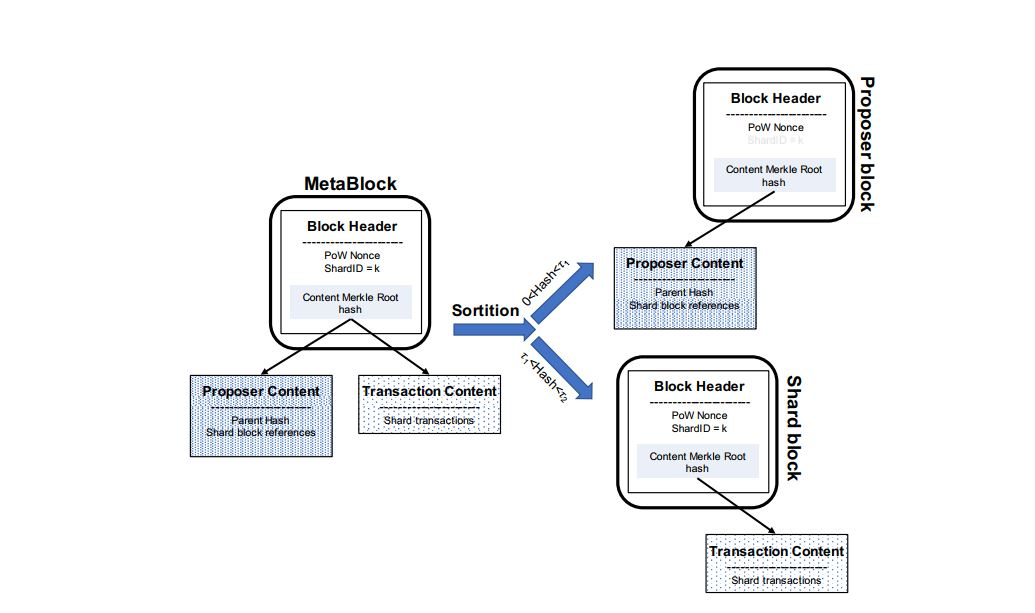
\includegraphics[width=0.8\linewidth]{Fig/10/F3}
        \caption{Uniconsensus architecture: 2-for-one PoW sortition.}
        \label{fig:f3}
    \end{figure}
\end{center}
Indeed, the uni-consensus architecture offers significant improvements in resource usage and scalability compared to traditional full replication blockchains. By allowing each node to maintain only the proposer block tree and a shard ledger of its choice, the system achieves better efficiency. Nodes are no longer burdened with maintaining the ledgers of all $K$ shards, but only a fraction $\frac{1}{K}$, which reduces storage, computation, and communication requirements.\\
One notable advantage of the uni-consensus architecture is that it does not require a majority of honest nodes in each shard to maintain safety. This means that the system remains secure even when a shard has less than a majority of honest nodes. In such cases, adversarial nodes in the shard cannot alter the log of shard blocks without violating the safety properties of the consensus engine. Since all nodes participate in the main consensus engine, any malicious attempt to tamper with shard blocks would be quickly detected and rejected by the honest majority in the main consensus engine.\\
The elimination of the need for a consensus majority in each shard significantly strengthens the security of the uni-consensus architecture, making it safe against a fully adaptive adversary. Even with less than a majority of honest nodes in some shards, the overall security and integrity of the system are maintained, ensuring the resilience of the blockchain against various adversarial attacks.\\
The uni-consensus architecture addresses several limitations of the multi-consensus approach and offers several key advantages:
\begin{enumerate}
    \item \textbf{Identity-free sharding:} Unlike the multiconsensus architecture, the uniconsensus architecture does not require an N2S allocation for nodes. Nodes are free to join any shard of their choice without the need for an on-chain validator/miner identity. This reduces complexity and allows for greater flexibility in node participation.
    \item \textbf{Small number of nodes per shard:} Since the uni-consensus architecture does not rely on an honest majority within each shard, the constraint on the number of nodes per shard, as depicted in Figure \ref{fig:f1}, no longer applies. This allows for a more scalable and efficient allocation of nodes across shards.
    \item \textbf{Adaptive adversary resistance:} The uni-consensus architecture is resilient to safety violations by corrupting a shard. Since the presence of an honest majority within a shard is no longer a requirement for security, destroying an honest majority in a shard is not a viable attack strategy. Additionally, the lack of an on-chain mapping of miner identity to shard ID weakens the targeting capabilities of adaptive adversaries.
\end{enumerate}
However, the self-allocation of nodes in the uni-consensus architecture can lead to potential liveness attacks. An adversary could concentrate its mining power on a single shard, overwhelming honest shard blocks and reducing the fraction of honest blocks in the shard. This could throttle the throughput of honest transactions in the targeted shard, causing a loss in liveness.\\
To prevent such liveness attacks, a dynamic self-allocation (DSA) algorithm like Free2Shard can be employed. DSA allows honest nodes to respond to adversarial actions by relocating themselves to shards with low throughput, possibly due to liveness attacks. Such relocation is incentivized by higher transaction fees in shards with low throughput. By allowing nodes to dynamically self-allocate based on current conditions, DSA enhances the system's resilience to liveness attacks and maintains a more balanced and efficient distribution of nodes across shards.
\section{ Bootstrap and State-commitment}
In both the multiconsensus and uniconsensus architectures, when an honest node decides to relocate to a new shard, it needs to efficiently download and verify the state of that shard. This process is akin to bootstrapping in a blockchain context. However, simply processing the entire ledger of the new shard would negate the scaling benefits of sharding since the node would end up processing the ledgers of all shards eventually.\\
To address this issue and enable efficient relocation to a new shard, the concept of trusted state-commitments is introduced. State-commitments are accumulators of a ledger's state that are universally agreed upon by all nodes in the network to be correct. They serve as cryptographic proofs of the validity of the ledger's state. When a bootstrapping node joins a new shard, it can download the latest state of that shard and verify its correctness using the state-commitments.\\
The accumulator used for state-commitments is a cryptographic data structure that efficiently allows for the inclusion of new data (transactions) while providing proof that a particular element (state) is a part of the accumulator. By relying on these state-commitments, the bootstrapping node can trustlessly verify the state without relying on any single node in the new shard, ensuring security and integrity.\\
The process of generating and maintaining these state-commitments is crucial for the functioning of the sharding architecture. Properly designed state-commitments enable efficient and secure bootstrapping for nodes relocating to new shards, ensuring that the benefits of sharding in terms of scaling and efficiency are preserved.
\subsection{Accumulator for State-commitments}
To design an accumulator for the (account, value) tuples in the ledger's state, a sparse Merkle tree is used. In a sparse Merkle tree, there exists a leaf in the tree for every possible output from a cryptographic hash function, representing every possible account number in the ledger. However, most of the leaves are empty, making the tree sparse. This allows for efficient simulations because only the non-empty leaves need to be stored and updated.\\
Unlike a regular Merkle tree, an ordered Merkle tree is not used for state-commitments because it is costly to add or remove accounts from the middle of the tree, especially when the tree is large.\\
In the sparse Merkle tree, the value of a leaf is the balance of the corresponding account if it exists or null if the account does not exist. This way, the tree can efficiently represent the dynamic nature of the ledger's state with insertions and deletions of accounts.\\
To further optimize the sparse Merkle tree, a compressed form called Merkle Patricia Trie (MPT) is often used. MPT has similar insertion and deletion complexity ($O(1)$) as a sparse Merkle tree but is more space-efficient, A sparse merkle tree with only two accounts is illustrated in Figure \ref{fig:f4}.\\
A state commitment consists of the root of the Merkle Patricia Trie representing a shard's execution state. This root is generated at regular intervals known as epochs and is posted on either the beacon chain (for multiconsensus architecture) or the main consensus engine (for uniconsensus architecture). By having all nodes agree on the state commitment's root, the validity and consistency of the ledger's state can be ensured across the network, enabling secure and efficient bootstrapping for nodes relocating to new shards.
\begin{center}
    \begin{figure}
        \centering
        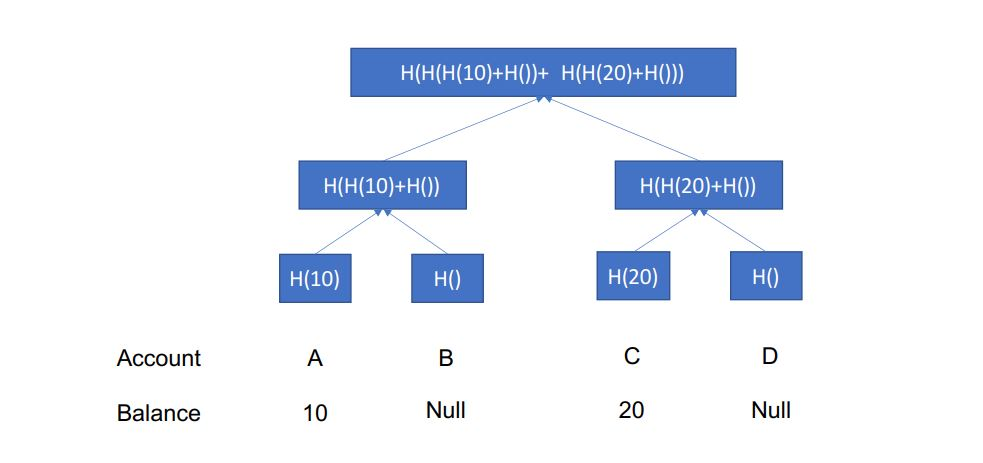
\includegraphics[width=0.8\linewidth]{Fig/10/F4}
        \caption{State-commitment using a sparse Merkle tree.}
        \label{fig:f4}
    \end{figure}
\end{center}
\subsection{Generation and agreement on state commitments}
Ensuring that state commitments are generated and agreed upon in a Byzantine fault-tolerant manner is crucial for the security and integrity of the system. In both the multiconsensus and uniconsensus architectures, the process of posting state-commitments must be resistant to attacks and manipulations by adversaries. This focuses on the following discussion:
\begin{enumerate}
    \item \textbf{Multiconsensus:} Indeed, the multiconsensus architecture benefits from the strong underlying assumptions of node identity and an honest majority within each shard. With these assumptions in place, the process of state-commitment generation becomes straightforward.\\
    Each shard in the multi-consensus architecture can generate a state-root representing the state of the shard at a particular point in time. This state root is then signed by a majority of the nodes within that shard, effectively turning it into a state-commitment. The fact that a majority of nodes in the shard sign the state root provides a strong level of trust and ensures the correctness of the state-commitment.\\
    State-commitments can be treated as regular transactions on the shard itself, subject to deterministic validation rules. This means that the execution state at the point in the ledger corresponding to the state-commitment must match the state represented by the commitment. This further reinforces the correctness and consistency of state-commitments.\\
    To facilitate the availability of the latest state-commitments for incoming nodes from different shards, these commitments are periodically posted on the beacon chain. This ensures that all nodes in the network can easily access and verify the state-commitments without relying on centralized sources. Since state-commitments are small in size (usually just the output of a cryptographic hash), posting them on the beacon chain incurs minimal overhead.
    \item \textbf{Uniconsensus} In the uniconsensus architecture, state-commitment generation is more intricate due to the absence of node identity and the lack of an assumption that each shard has an honest majority. Additionally, not all transactions included in the ledger are assumed to be valid, as validation is decoupled from ordering. This means that transaction validation occurs after the order of transactions has been agreed upon, making it challenging to verify the state-commitments across the entire network without defeating the purpose of sharding.\\
    To address these challenges, the uniconsensus architecture incorporates two novel ideas: interactivity among the nodes generating state-commitments and relying on honest nodes to detect fraud in the broadcasts, rather than proving the veracity of each broadcast.\\
    The state-commitments are generated by specific parties within a shard, known as commitment leaders. The broadcasts of these state-commitments are scrutinized for fraud by the honest nodes in the shard. If any fraud is detected, an honest node, referred to as the challenger, posts a proof of fraud on the main consensus engine, the proposer chain. If no fraud-proof is posted within a specific time frame, the state-commitment is assumed to be honest.\\
    To keep the proposer chain lightweight, the fraud proof must also be lightweight. Since consecutive state-commitments summarize thousands of transactions, it is not desirable for the consensus engine to process all those transactions to verify a fraud-proof. Instead, the goal is to pinpoint the fraud-proof of incorrect computation to just one transaction or bytecode. This is achieved through a logarithmic search across all transactions.\\
    The process is illustrated in Figure \ref{fig:f5}a, where the fraud-proof is generated by a challenger and posted on the proposer chain to challenge the correctness of a state-commitment.\\
    By employing interactivity and relying on honest nodes to detect fraud, the uni-consensus architecture establishes a fraud-proof based approach for state-commitments. Assuming correct if not proven wrong within a time frame allows for an efficient and secure generation of state-commitments, even in the absence of node identity and an honest majority within each shard.
    \begin{center}
        \begin{figure}
            \centering
            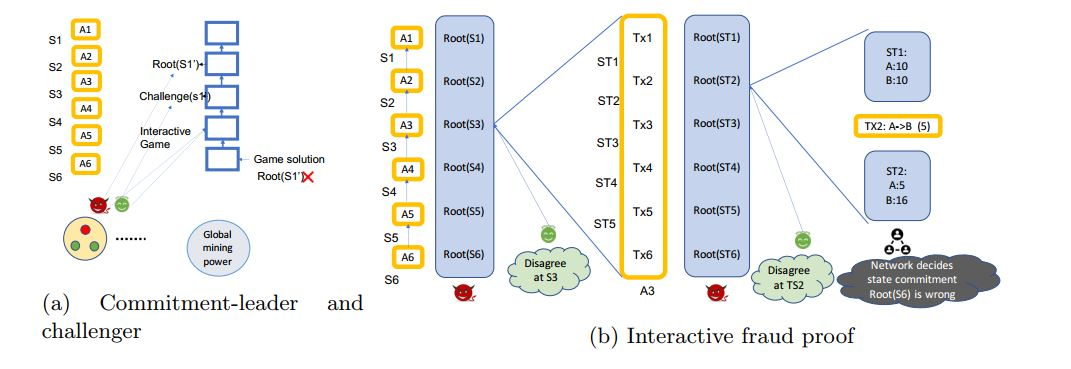
\includegraphics[width=0.8\linewidth]{Fig/10/F5}
            \caption{State-commitment in uni-consensus architecture.}
            \label{fig:f5}
        \end{figure}
    \end{center}
    The logarithmic fraud search mechanism involves two parties, a commitment-leader, and a challenger, both belonging to the same shard. When the commitment-leader, who is adversarial, posts an invalid state-commitment on the consensus engine, the challenger detects the fraud and initiates the fraud search protocol. The following sequence of interactions summarizes the protocol once fraud is detected and challenged:\\
    \begin{enumerate}
        \item The commitment-leader posts intermediate states for the challenged state, attempting to prove the validity of their state-commitment.
        \item The challenger responds with a number indicating the first intermediate state where their view differs from that of the leader.
        \item The protocol continues to the next round, with the commitment-leader posting intermediate states for the smaller challenged state, and the challenger responding based on the previous step.
        \item The interactions proceed in a recursive manner until the conflict is resolved down to a single transaction. At this point, the search for a single transaction is complete.
        \item The identified transaction is posted on the consensus engine to decide if fraud has occurred or not. If the transaction is indeed invalid, it is removed from the ledger, and consensus is regained.
    \end{enumerate}
    The process is illustrated in Figure \ref{fig:f5}b, where the fraudulent state-commitment is challenged, and the protocol recursively searches for the specific transaction that caused the fraud.\\
    Once fraud has been detected and the incriminating transaction is found, it is excised from the ledger, and consensus is restored. In some designs, the commitment-leader may also be penalized for this fraudulent behavior. For example, in a Proof of Work (PoW) setting, the penalty can be imposed outside the blockchain. In the context of Proof of Stake (PoS) mechanisms, the penalization can be handled within the blockchain, such as slashing a collateral transaction required to be posted by the commitment-leaders.\\
    The fraud-proof mechanism, along with the ability to penalize adversarial behavior, incentivizes commitment-leaders to follow the protocol honestly, as they risk losing rewards or collateral if they engage in fraudulent activities. This approach ensures the integrity and security of state-commitments in the uni-consensus architecture.
\end{enumerate} 
\section{Cross-shard transactions}
The single-stage cross-shard transaction protocol presented above, while seemingly suitable for ensuring atomicity, does not actually achieve it due to a violation that arises in certain scenarios. Specifically, if funds $x_{B}$ are not available in shard B, the protocol fails to ensure atomicity.\\
In this scenario, when the transaction is initiated, shard A successfully locks $x_{A}$ and reflects this in its state commitment $S1_{A}$. However, shard B cannot lock $x_{B}$ since those funds do not exist. As a result, a proof of lock from both input shards is not available for the cross-shard transaction. Consequently, output shards C and D do not release funds $y_{C}$ and $y_{D}$. The fund $x_{A}$ remains locked indefinitely, causing the transaction to be committed in shard A while being aborted in the rest of the shards. This inconsistency breaks atomicity.\\
To address this limitation and ensure atomicity in cross-shard transactions, a two-stage commit protocol can be utilized. The protocol involves the following steps:\\
\begin{enumerate}
    \item Input shards (A and B in the example) initiate the transaction and lock the funds $x_{A}$ and $x_{B}$ for this cross-shard transaction. However, instead of directly updating their state commitments, they first create a provisional transaction record that indicates the intent to participate in the cross-shard transaction.
    \item Output shards (C and D) receive the provisional transaction records from input shards and verify their validity, ensuring that the funds $x_{A}$ and $x_{B}$ are indeed locked.
    \item Once the output shards are assured of the locks, they create their own provisional transaction records, indicating the receipt of funds $y_{C}$ and $y_{D}$.
    \item The output shards send a confirmation back to the input shards, acknowledging that they have successfully received the provisional transaction records and are ready to proceed.
    \item Upon receiving the confirmation, the input shards finalize the transaction by updating their state commitments to reflect the lock of funds $x_{A}$ and $x_{B}$.
    \item Finally, the output shards also finalize the transaction by updating their state commitments to include the funds $y_{C}$ and $y_{D}$.
\end{enumerate}
By using a two-stage commit protocol, atomicity can be ensured in cross-shard transactions. The protocol ensures that if the transaction is committed (aborted) in one shard, it will be committed (aborted) in all participating shards, avoiding any inconsistencies and preserving the integrity of the overall transaction.
\begin{center}
    \begin{figure}
        \centering
        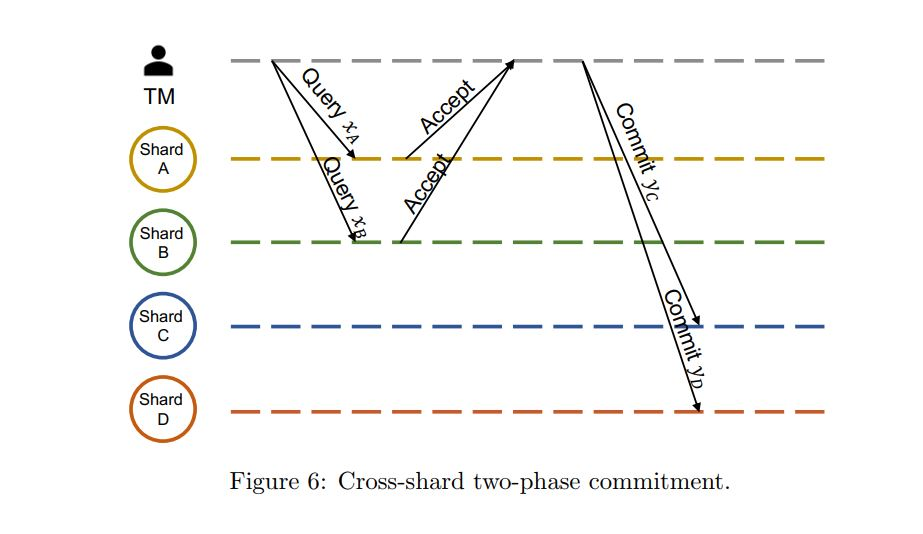
\includegraphics[width=0.8\linewidth]{Fig/10/F6}
        \caption{Cross-shard two-phase commitment.}
        \label{fig:f6}
    \end{figure}
\end{center}
The generalized two-phase commitment protocol presented above ensures atomicity in cross-shard transactions by allowing a rollback of the transaction if any of the input shards fail to lock the required funds. The protocol works as follows:\\
\textbf{Phase 1:}\\
\begin{itemize}
    \item A transaction manager (TM) is designated to read state commitments across shards. Typically, the TM represents the spending party/parties.
    \item If the input funds $x_{A}$ and $x_{B}$ are available in shard A and B, respectively, both shards update their state to lock the funds, indicating that they are reserved for the cross-shard transaction.
    \item If an input fund in shard A is not available (i.e., funds $x_{A}$ are not present), shard A updates its state to mark fund $x_{A}$ as unavailable by adding a receipt of unavailability to its state.
\end{itemize}
\textbf{Phase 2:}\\
\begin{itemize}
    \item Once the TM confirms that the funds are locked in all input shards, as indicated by state commitments $S1_{A}$ and $S1_{B}$, it sends a proof of lock to the output shards (shards C and D).
    \item Upon receiving the proof of lock, the output shards generate the funds $y_{C}$ and $y_{D}$ for the cross-shard transaction and update their state commitments accordingly.
\end{itemize}
If the TM observes that funds are unavailable in any of the input shards (based on state commitments $S1_{A}$ and $S1_{B}$), it takes the necessary action to ensure atomicity:\\
\begin{itemize}
    \item The TM sends a rollback transaction to all input shards, consisting of a proof of receipt of unavailability from one of the input shards.
    \item The rollback transaction prompts the input shards to release any locked funds (e.g., $x_{A}$) that were reserved for the cross-shard transaction.
\end{itemize}
By using this two-phase commitment protocol with a possibility of rollback, atomicity is guaranteed. The protocol ensures that either all the input funds of the transaction are successfully spent (locked) in their respective shards, or the entire transaction is aborted, and any locked funds are reclaimed.\\
In the example scenario discussed earlier, where funds $x_{B}$ are not available in shard B, the two-phase commitment protocol ensures that the transaction is aborted in all participating shards. Once shard A locks $x_{A}$ and shard B marks $x_{B}$ as unavailable, the TM can initiate a rollback transaction to unlock $x_{A}$ in shard A, ensuring that the entire transaction is aborted consistently across all shards. This avoids any partial spending of input funds and maintains the integrity of the cross-shard transaction.
